% Slide 16: Geometry Calibration (NEW)
\begin{frame}{Geometry is hard even for well-prepared humans}
  \begin{center}
    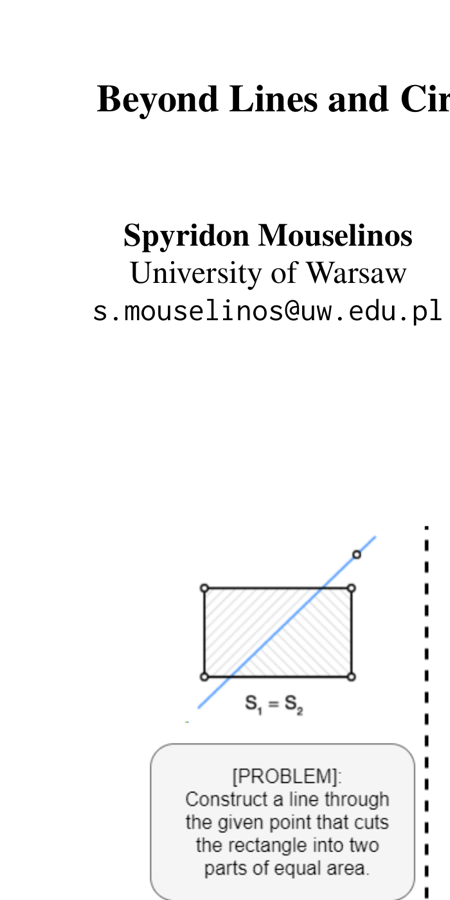
\includegraphics[width=0.6\textwidth,height=0.6\textheight,keepaspectratio]{assets/euclidea-problem-screenshot}
  \end{center}

  \vspace{1em}

  \begin{center}
    \colorbox{yellow!20}{%
      \begin{minipage}{0.7\textwidth}
        \centering
        \Large
        \textbf{Human study performance: 30.5\%}
      \end{minipage}
    }
  \end{center}

  \vspace{1em}

  \begin{center}
    This is why geometry is the right culmination of the thesis.
  \end{center}

  \note{Before I show you the model results, let me calibrate you. We ran a human study on 20 Euclidea problems. Well-prepared participants averaged 30.5\%. This is not a toy benchmark - it's genuinely hard geometric reasoning.}
\end{frame}
